\chapter{Úvod}

USB je najrozšírenejšia zbernica na pripojenie rôznych periférií k počítaču. Vznikla v druhej polovici 90. rokov 20. storočia, kedy boli rôzne zariadenia a ich porty veľmi úzko mapované. Na pripojenie základných zariadení ako myš alebo klávesnica slúžil napríklad sériový port PS/2~\cite{ps2_port}. K pripojeniu tlačiarne sa často používal paralelný port Centronics~\cite{parallel_port}. Ešte pred PS/2 portom sa myš pripájala cez veľmi známy sériový port RS-232~\cite{rs232_port}. Všetky tieto porty boli typu \textit{point-to-point} -- na jeden port je možné pripojiť len jedno zariadenie. Toto sa paralelným portom dalo čiastočné obísť tým, že niektoré zariadenia podporovali tzv. \textit{daisy chain} -- do pripojeného zariadenia sa pripojí ďalšie zariadenie, do toho sa pripojí ďalšie, atď. (napríklad typická tlačiareň toto nepodporovala, takže musela byť pripojená na konci \textit{daisy chainu}). Existovala takisto paralelná \textit{SCSI} zbernica~\cite{scsi_hub}, ktorej návrh bol prispôsobený aby podporoval  \textit{daisy chain}. Tá fungovala dobre na zariadeniach ako externé HDD a skenery, ale bola nepraktická pre zariadenia ako myš a klávesnica.

USB vzniklo za účelom nahradiť a zjednotiť tieto spôsoby pripojenia bežných periférií k počítaču. Návrh zbernice je založený na hviezdicovej topológii, ktorá umožňuje cez jeden port pripojiť až 127 zariadení súčasne. Z toho vyplýva, že USB interface v sebe zahŕňa obrovskú množinu protokolov, ktoré sú hierarchicky usporiadané. K analýze paketov ktoré sa pohybujú na danej zbernici nám slúžia tzv. USB paket analyzátory, ktoré môžu mať podobu hardwarového zariadenia alebo softwarovej aplikácie. Môžu slúžiť napríklad ako učebná pomôcka pre účel lepšieho pochopenia jednotlivých protokolov. Takisto sa často využívajú pri implementácii vlastného USB zariadenia na ladenie komunikácie medzi daným zariadením a driverom. Využitie ale majú aj v opačnom prípade, keď implementujeme vlastný driver a potrebujeme sledovať jeho komunikáciu s konkrétnym zariadením. Cieľom tejto práce bude naprogramovať funkčný softwarový USB analyzátor, ktorý by mal presnejšie slúžiť práve ako učebná pomôcka pre lepšie pochopenie určitej množiny protokolov. Cieľová platforma aplikácie bude Windows.

\section{Základné pojmy}
\label{uvod:sec:zakl_pojmy}
V tejto sekcii si vysvetlíme niektoré základné pojmy ktoré budeme neskôr v~texte používať.

\begin{figure}[!htb]
	\centering
	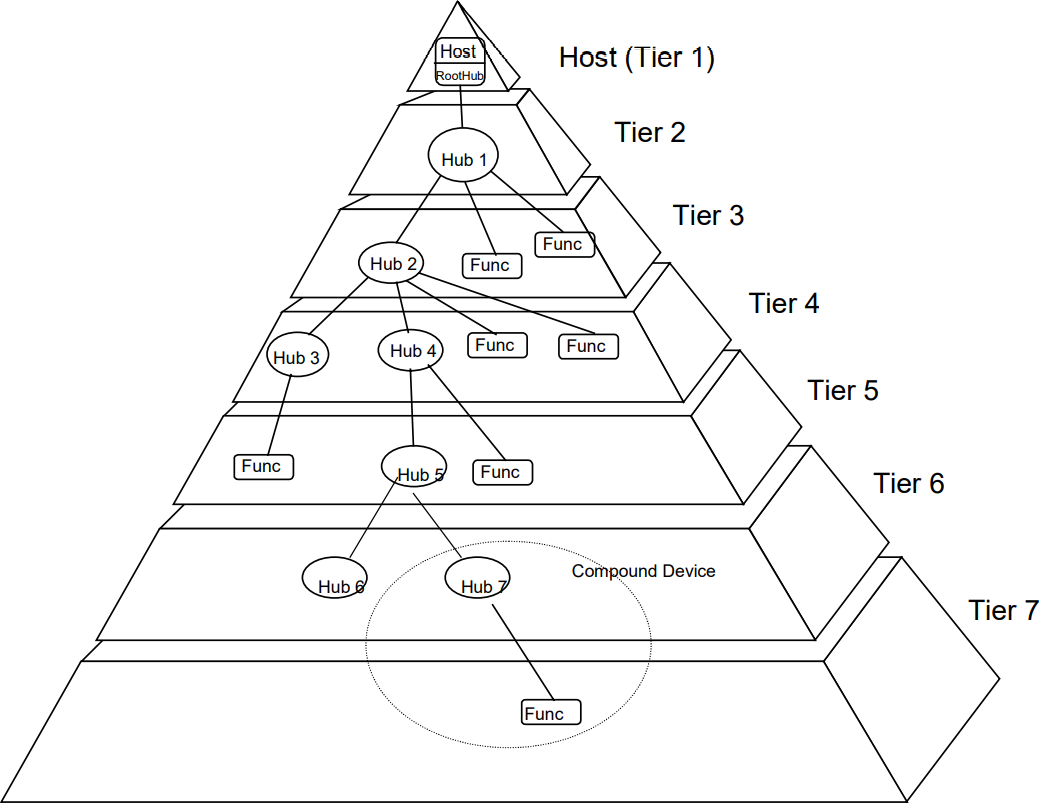
\includegraphics[width=\textwidth]{img/uvod_usb_topology}
	\caption{USB topológia. Obrázok prevzatý z USB 2.0 špecifikácie~\cite{usb_topology}.}
	\label{obr:uvod:usb_topology}
\end{figure}

Ako sme už vyššie spomínali a ako ilustruje obrázok~\ref{obr:uvod:usb_topology}, USB zbernica je založená na vrstevnatej hviezdicovej topológii. Na vrchu všetkého sa nachádza \textbf{USB Host}~\cite{usb_host}, čo je systém do ktorého sa pripájajú ostatné USB zariadenia (v našom prípade je \textit{USB Host} počítač). \textbf{USB zariadenie}~\cite{usb_device} je buď:
\begin{itemize}
\item \textbf{Hub}~\cite{usb_hub} -- poskytuje dodatočné pripojenia k USB zbernici.
\item \textbf{Funkcia}~\cite{usb_function} -- poskytuje novú funkcionalitu systému (napríklad joystick, reproduktory, myš a pod.)
\end{itemize}

 V každom USB systéme sa nachádza práve jeden \textit{USB Host}. Ten má integrovaný tzv. \textbf{Root Hub}~\cite{usb_host}, ktorý poskytuje možné body pripojenia pre ďalšie zariadenia. Interface medzi hostom a USB sa nazýva \textbf{Host Controller}~\cite{usb_host}. Vzhľadom na niektoré časové obmedzenia USB je maximálny počet vrstiev 7 (vrátane \textit{USB Host} vrstvy). Každý káblový segment je \textit{point-to-point}~\cite{usb_bus_topology} spojenie medzi:
\begin{itemize}
\item \textit{host} $\longleftrightarrow$ \textit{hub}/\textit{funkcia}
\item \textit{hub} $\longleftrightarrow$ \textit{hub}/\textit{funkcia}
\end{itemize}

USB zariadenia využívajú tzv. \textbf{descriptory} na predávanie informácií o sebe samých. \textbf{Descriptor}~\cite{usb_descriptor} je dátová štruktúra s predom definovaným formátom. Existuje viacero typov \textit{USB descriptorov} (device, endpoint, interface atď.), ktorých význam si vysvetlíme neskôr.

Vzhľadom na hierarchickú štruktúru USB protokolov sa \textit{USB zariadenia} delia na rôzne triedy~\cite{usb_classes}. \textit{USB trieda} je zoskupenie zariadení (alebo interfacov) ktoré majú spoločné vlastnosti alebo funkcionalitu. Tieto triedy umožňujú \textit{USB hostovi} identifikovať dané zariadenie a jeho funkcionalitu. Každá trieda má svoju vlastnú \textit{Class Specification} -- definuje správanie zariadení v jednotlivých triedach a opisuje ich komunikačný protokol, ktorý sa naprieč triedami líši. Takisto definuje rôzne descriptory, ktoré sú špecifické pre danú triedu. Príklady USB tried a jednotlivých zariadení ktoré do nich patria sú:
\begin{itemize}
\item Mass Storage (napr. SD karta a flash disk)
\item Audio (napr. reproduktory a slúchadlá)
\item HID -- Human Interface Device (napr. myš, klávesnica alebo joystick)
\end{itemize}

\textbf{Paket}~\cite{usb_packet} je súbor dát zoskupený na prenos po zbernici. Typicky sa skladá z troch častí:
\begin{itemize}
\item základné informácie o danom pakete (napríklad zdroj, cieľ, dĺžka) -- takisto nazývané hlavička paketu
\item samotné dáta
\item detekcia chýb, opravné bity
\end{itemize}

Komunikácia na zbernici medzi \textit{USB hostom} a \textit{zariadením} prebieha práve pomocou prenosu \textit{USB paketov}.   Existujú 4 typy takýchto prenosov~\cite{usb_type_transfers}:
\begin{itemize}
\item \textbf{Control Transfer} -- používa sa na konfiguráciu \textit{USB zariadenia} v momente keď sa pripojí na zbernicu.
\item \textbf{Bulk Data Transfer} -- typicky pozostáva z väčšieho množstva dát ktoré sú posielané nárazovo (využívajú ho najmä tlačiarne alebo skener). Vďaka detekcii chýb na hardwarovej úrovni je zaistená správnosť prenesených dát.
\item \textbf{Interrupt Data Transfer} -- spoľahlivý prenos ktorý sa využíva hlavne na odovzdávanie aktuálnych informácií (ako napríklad pohyb myšou). Tieto informácie musia byť doručené USB zbernicou za čas kratší ako má špecifikované dané zariadenie.
\item \textbf{Isochronous Data Transfer} -- takisto nazývaný ako streaming v reálnom čase. Typický príklad je prenos zvuku.
\end{itemize}

Našu aplikáciu by sme chceli zamerať na Windows a tak si vysvetlíme ešte zopár špecifických pojmov, ktoré sa viažu na túto kokrétnu platformu.

Podľa MSDN dokumentácie~\cite{usbclientdriver} je \textbf{USB client driver} software nainštalovaný na počítači, ktorý komunikuje s USB zariadením aby spojazdnil jeho funkcionalitu. Žiaden \textit{USB client driver} ale nemôže priamo komunikovať so svojím zariadením. Namiesto toho vytvorí požiadavku, súčasťou ktorej je dátová štruktúra nazývaná \textbf{URB}~\cite{usburb} (USB Request Block). Tá opisuje detaily požiadavku, takisto ako aj status o jeho vykonaní.

Na záver si ešte zadefinujeme rozdiel medzi \textit{USB paket analyzátorom} a \textit{USB paket snifferom}. Pod pojmom \textbf{USB paket sniffer} budeme rozumieť aplikáciu, ktorá monitoruje dianie na USB zbernici a je schopná ho rozumným spôsobom ukladať v predom definovanom formáte. Ako \textbf{USB paket analyzátor} budeme brať aplikáciu ktorá je schopná rozanalyzovať USB pakety (istým spôsobom ich vyobraziť alebo ukázať ich sémantický význam) uložené v predom definovanom formáte. Bežne sa tieto pojmy označujú za jednu a tú istú vec, aj keď ich funkcionalita spolu nijako priamočiaro nesúvisí a existujú nástroje, ktoré vedia len jedno alebo druhé. Preto dáva zmysel ich od seba explicitne oddeliť.

Momentálne by sme mali chápať všetky základné pojmy týkajúce sa USB, a tak si poďme trochu bližšie objasniť zameranie našej aplikácie. Našu aplikáciu zameriavame výukovým smerom pre programátorov, ktorí chcú lepšie pochopiť komunikáciu na USB zbernici. Z toho dôvodu by sme v nej určite chceli zahrnúť analýzu základných USB descriptorov, ktoré sú bližšie definované v špecifikácii USB 2.0~\cite{usbdoc} v~kapitole 9.6. Keďže chceme bližšie priblížiť komunikáciu na danej zbernici, potrebujeme konkrétne zariadenia, s ktorými ju budeme analyzovať. Dáva dobrý zmysel si zvoliť zariadenia, ktoré každý z nás dobre pozná, má ich k dispozícii a bežne ich využíva. Zároveň by ale mali mať dostatočne jednoduchý komunikačný protokol. Práve preto sa s našou aplikáciou zameriame na užšiu podmnožinu HID zariadení, konkrétne myš, klávesnica a joystick. Vzhľadom na zameranie našej aplikácie výukovým smerom prikladáme najväčšiu prioritu samotnej analýze dát.  Z dôvodu celkovej univerzality USB je z didaktického hľadiska ťažké nasimulovať jednotný príklad u každého študenta zvlášť. Už len obyčajná myš, aj keď je to jedno zariadenie, má od rôznych výrobcov inak nadefinované správanie a posiela dáta v rozličných formátoch. Preto je pre nás dôležité vedieť analyzovať pakety, ktoré si učiteľ predpripraví, skontroluje ich didaktickú správnosť a uloží do súboru. Podpora živého zachytávania paketov a ich analýzy je tak v našom programe najmenej dôležitá.

Keďže sa v našej práci budeme venovať hlavne analýze HID zariadení, tak si túto USB triedu rozoberieme trochu detailnejšie.

\subsection*{HID}
\label{uvod:sec:HID}

Podľa dodatku k USB špecifikácii~\cite{usbhid} je \textbf{HID} (z anglického \uv{Human Interface Device}) USB trieda pozostávajúca prevažne zo zariadení, ktoré sú využívané človekom na riadenie určitých systémovových aplikácií. Medzi najpoužívanejšie príklady patrí myš, klávesnica alebo joystick.

Ako sme už spomínali vyššie, jednotlivé USB triedy majú definované vlastné descriptory špecifické pre danú triedu. Jedným z takýchto descriptorov je aj \textit{Report Descripor}, ktorý popisuje dáta generované konkrétnym zariadením. Analýzou \textit{Report Descriporu} sme schopní určiť veľkosť a kompozíciu dát posielaných zariadením. Z toho vyplýva, že komunikácia HID zariadenia s USB hostom sa môže líšiť nie len vo veľkosti posielaných dát, ale takisto aj v ich význame.

Lepšie to uvidíme na konkrétnom príklade. K dispozícii máme 2 rozdielne myši (obrázok~\ref{obr:uvod:mysi:porovnanie}) -- Genius DX\=/120~\cite{genius_mouse} a Logitech G502 Proteus Spectrum~\cite{logitech_mouse}

\begin{figure}[!htb]
\centering
\begin{subfigure}{.5\textwidth}
  \centering
  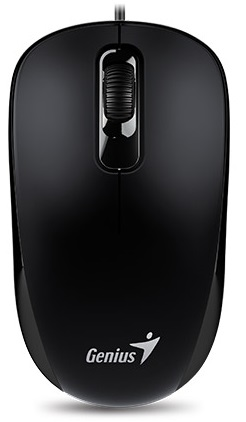
\includegraphics[width=.4\linewidth]{img/genius_mys.jpg}
  \caption{Fotka genius myši prevzatá z oficiálnej genius stránky~\cite{genius_mouse_pic}}
  \label{obr:uvod:genius:mouse:pic}
\end{subfigure}%
\begin{subfigure}{.5\textwidth}
  \centering
  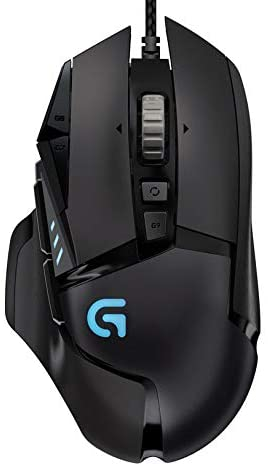
\includegraphics[width=.4\linewidth]{img/logitech_mys}
  \caption{Fotka logitech myši prevzatá zo stránky obchodu~\cite{logitech_mouse_pic}}
  \label{fig:sub2}
\end{subfigure}
\caption{Ukážka myší, ktorých input budeme porovnávať}
\label{obr:uvod:mysi:porovnanie}
\end{figure}

Teraz si ukážeme ako sa líši ich input. Dáta budeme vyobrazovať pomocou obyčajného hexdumpu (zvýraznená časť v hexdumpe reprezentuje input zariadenia). Na oboch myšiach budeme mať stlačené ľavé tlačidlo a mierne ich posunieme smerom hore. Dáta, ktoré poslala Genius myš sú vyobrazené na obrázku~\ref{obr:uvod:genius:input} a dáta poslané Logitech myšou môžeme vidieť na obrázku~\ref{obr:uvod:logitech:input}. Už na prvý pohľad môžeme vidieť, že dáta majú rozdielnu dĺžku a obecne o ich význame nevieme nič povedať -- ten je definovaný v \textit{Report Descriptore}.

\begin{figure}[!htb]
	\centering
	
\includegraphics[width=12cm]{img/uvod_genius_input}
	\caption{Ukážka hexdumpu so zvýrazneným inputom Genius myši.}
	\label{obr:uvod:genius:input}
\end{figure}

\begin{figure}[!htb]
	\centering
	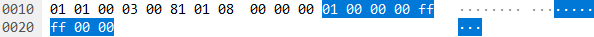
\includegraphics[width=12cm]{img/uvod_logitech_input}
	\caption{Ukážka hexdumpu so zvýrazneným inputom Logitech myši.}
	\label{obr:uvod:logitech:input}
\end{figure}

Aj napriek tomu, že sa jedná o zariadenia z tej istej USB triedy a dokonca o rovnaké zariadenie -- myš,  má ich komunikácia rozličný tvar definovaný priamo výrobcom zariadenia. Analýzou \textit{Report Descriporu} (o ktorej si viac povieme v sekcii~\ref{kap03:sec:report_desc}) sme zistili, že dáta, ktoré poslala Genius myš majú nasledujúci význam:
\begin{itemize}
\item Byte 0: bity 0--2 reprezentujú stlačenie jednotlivých tlačidiel, bity 3--7 tvoria len dodatočnú výplň bytu
\item Byte 1: reprezentuje súradnicu X
\item Byte 2: reprezentuje súradnicu Y
\item Byte 3: reprezentuje koliesko myši
\end{itemize}

Pre porovnanie, význam dát poslaných Logitech myšou je nasledovný:
\begin{itemize}
\item Byte 0--1: reprezentujú stlačenie jednotlivých tlačidiel
\item Byte 2--3: reprezentuje súradnicu X
\item Byte 4--5: reprezentuje súradnicu Y
\item Byte 6: reprezentuje koliesko myši
\item Byte 7: je rezervovaný výrobcom myši
\end{itemize}

Vizuálne zobrazený význam dát Genius myši je ukázaný na obrázku~\ref{obr:uvod:genius:input:vyznam} a Logitech myši na obrázku~\ref{obr:uvod:logitech:input:vyznam}.

\begin{figure}[!htb]
	\centering
	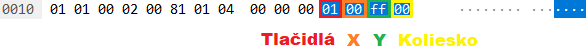
\includegraphics[width=12cm]{img/uvod_genius_input_vyznam}
	\caption{Ukážka hexdumpu so zvýrazneným inputom Genius myši s významom.}
	\label{obr:uvod:genius:input:vyznam}
\end{figure}

\begin{figure}[!htb]
	\centering
	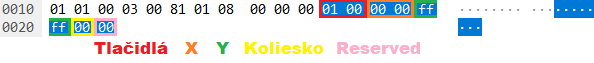
\includegraphics[width=12cm]{img/uvod_logitech_input_vyznam}
	\caption{Ukážka hexdumpu so zvýrazneným inputom Logitech myši s významom.}
	\label{obr:uvod:logitech:input:vyznam}
\end{figure}

Z toho vyplýva, že aby sme boli schopní vykonať sémantickú analýzu HID zariadení, bude pre nás kľúčové vedieť rozparsovať \textit{Report Descripor} a na základe toho interpretovať input zariadení.

\section{Existujúce aplikácie}
\label{uvod:sec:existujuce_aplikacie}

Momentálne existuje niekoľko známych aplikácií ktoré slúžia na analýzu USB paketov. Ich predbežným skúmaním a používaním sme ale zistili, že úplne nevyhovujú našim konkrétnym požiadavkám. Avšak mnohé ich funkcie nám prídu užitočné a môžu poslúžiť ako inšpirácia v implementovaní našej aplikácie. V tejto kapitole si ukážeme výhody a nevýhody zopár aplikácií, ktoré sme si zvolili ako príklady v oblasti paket analyzátorov. Ich výber spočíval v tom, že sú veľmi rozšírené medzi verejnosťou a sú najbližšie k tomu čo by sme chceli od našej aplikácie.

Je nutné upozorniť, že väčšina dnešných analyzátorov sú platené aplikácie, prípadne majú odomknuté len základné vlastnosti s~možnosťou dokúpenia si plnej verzie. Práve preto sme nemali možnosť si pri všetkých vyskúšať ich celú funkcionalitu a na niektoré platené funkcie máme tak len ilustračný pohľad.


\subsection*{Wireshark}
\label{uvod:sec:Wireshark}

Aplikácia, ktorá na prvý pohľad nesúvisí s USB zbernicou. Wireshark je pravdepodobne najznámejší analyzátor a sniffer sieťových paketov. Jeho funkcionalita je veľmi rozsiahla, a~vzhľadom na~to, že sa jedná o~open-source projekt, neustále rastie. Vďaka jeho obecnému návrhu podporuje spoluprácu s~rôznymi inými sniffermi (LANalyzer, NetXRay a pod.). Jeden z~takýchto snifferov je \textit{USBPcap}, ktorý zachytáva USB komunikáciu a tým pádom je Wireshark schopný analyzovať pakety aj nad~touto zbernicou. 

Pre priblíženie niektorých funkcií Wiresharku si ukážeme analýzu komunikácie s USB myšou (Genius DX\=/120~\cite{genius_mouse})~\footnote{Verzia Wiresharku použítá v tejto sekcii na priblíženie jeho funkcionality je 3.2.6.}. Medzi tie úplne základné funkcie určite patrí hexdump dát nad~ktorými prebieha analýza, ktorý je vyobrazený na obrázku~\ref{obr:uvod:wireshark_hexdump}. 

\begin{figure}[!htb]
	\centering
	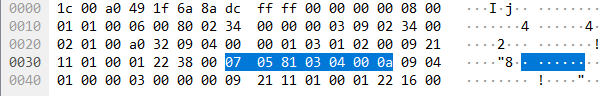
\includegraphics[width=12cm]{img/uvod_wireshark_hexdump}
	\caption{Ukážka hexdumpu vo Wiresharku.}
	\label{obr:uvod:wireshark_hexdump}
\end{figure}


Tento hexdump je tvorený dátami z jedného control prenosu, kde zariadenie posiela informácie o sebe samom v podobe rôznych descriptorov. 

V hexdumpe si takisto vieme pomocou kliknutia a ťahania myšou označiť ľubovoľné dáta, ktoré chceme. Zvýraznené byty na obrázku~\ref{obr:uvod:wireshark_hexdump_endpoint} reprezentujú jeden \textit{endpoint descriptor}.

\begin{figure}[!htb]
	\centering
	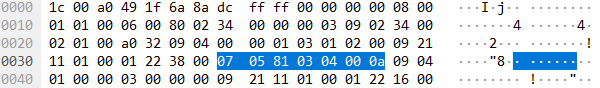
\includegraphics[width=12cm]{img/uvod_wireshark_hexdump_endpoint}
	\caption{Ukážka hexdumpu so zvýrazneným endpoint descriptorom.}
	\label{obr:uvod:wireshark_hexdump_endpoint}
\end{figure}

Pri pohybe myšou nad daným hexdumpom ponúka Wireshark interaktívnu odozvu, pričom farebne oddeľuje jednotlivé byty podľa ich významu. Na obrázku~\ref{obr:uvod:wireshark_hexdump_data_selection} vidíme konkrétny príklad -- ak podržíme myš nad hexa časťou bytu 00, automaticky nám to označí aj byte 04 pred ním, pretože spoločne reprezentujú jednotnú informáciu -- položku \textit{wMaxPacketSize} v \textit{endpoint descriptore}.

\begin{figure}[!htb]
	\centering
	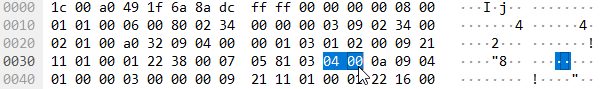
\includegraphics[width=12cm]{img/uvod_wireshark_data_selection}
	\caption{Ukážka hexdumpu s farebným oddelením na základe významu.}
	\label{obr:uvod:wireshark_hexdump_data_selection}
\end{figure}

Ďalšia užitočná vlastnosť je, že pri označení hexa znakov v hexdumpe, sa samé označia aj im odpovedajúce tlačiteľné znaky (obdobne to funguje aj opačným smerom). To, že vyššie označených 7 bytov na obrázku~\ref{obr:uvod:wireshark_hexdump_endpoint} reprezentujú \textit{endpoint descriptor} sme zistili vďaka špecifikácii jednotlivých descriptorov a vlastnou analýzou bytov v hexdumpe. Wireshark ale ponúka rozličné zobrazenie tých istých dát, a to napríklad aj pomocou stromovej štruktúry, ktorá už jednotlivým bytom pridáva ich sémantický význam v slovnom tvare ako je ukázané na obrázku~\ref{obr:uvod:tree_structure} nižšie.

\begin{figure}[!htb]
	\centering
	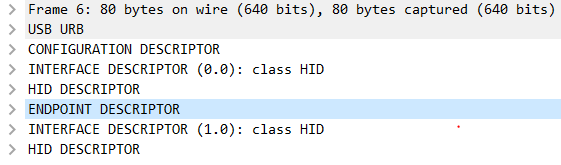
\includegraphics[width=11cm]{img/uvod_tree_structure}
	\caption{Ukážka reprezentácie dát pomocou stromovej štruktúry.}
	\label{obr:uvod:tree_structure}
\end{figure}

 Jednotlivé položky si môžeme bližšie rozbaliť. Napríklad vyššie zvýraznených 7 bytov reprezentujú konkrétny \textit{endpoint descriptor}, ktorý je ukázaný na obrázku~\ref{obr:uvod:endpoint}. Na tom istom obrázku si takisto môžeme všimnúť, že položka \textit{wMaxPacketSize} má hodnotu 4, čo je presne hodnota bytov 04 00, ktoré sme spomínali vyššie na obrázku~\ref{obr:uvod:wireshark_hexdump_data_selection}

\begin{figure}[!htb]
	\centering
	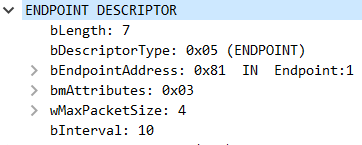
\includegraphics[width=8cm]{img/uvod_endpoint}
	\caption{Endpoint descriptor reprezentovaný dátami zvýraznenými na obrázku~\ref{obr:uvod:wireshark_hexdump} vyššie.}
	\label{obr:uvod:endpoint}
\end{figure}

Medzi viac špecifické funkcie patrí detailnejšie vyobrazenie jednotlivých bytov a~ich význam, ako je možné vidieť nižšie na~obrázku~\ref{obr:uvod:byte_detail_foto}. Na tomto obrázku vidíme rozbalenú položku \textit{bEndpointAddress}, ktorej hodnota je 0x81. Siedmy bit tejto hodnoty reprezentuje smer endpointu (IN -- slúži na prenos dát device $\longrightarrow$ host, OUT opačne) a dolné 4 bity označujú číslo endpointu. Túto vlastnosť aj napriek jej využitiu mnohé konkurenčné aplikácie postrádajú.

\begin{figure}[!htb]
	\centering
	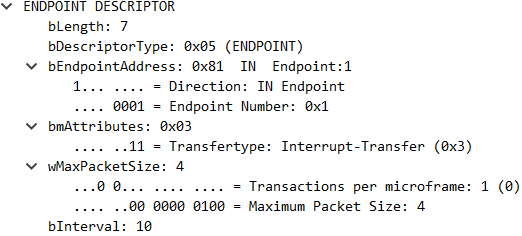
\includegraphics[width=8cm]{img/uvod_byte_detail}
	\caption{Ukážka vyobrazenia jednotlivých bytov.}
	\label{obr:uvod:byte_detail_foto}
\end{figure}

Wireshark ponúka interaktívne užívateľské rozhranie. V prípade kliknutia na konkrétny byte v hexdumpe sa nám označí jemu odpovedajúca položka v stromovej štruktúre. Príklad je ukázaný na obrázku~\ref{obr:uvod:hexdump_click}.

\begin{figure}[!htb]
	\centering
	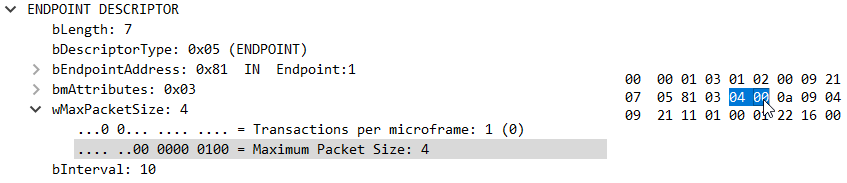
\includegraphics[width=\textwidth]{img/uvod_wireshark_hexdump_click}
	\caption{Ukážka kliknutia na položku v hexdumpe.}
	\label{obr:uvod:hexdump_click}
\end{figure}

Podobne to funguje aj opačne, takže ak klikneme na položku v stromovej štruktúre, označí sa jej odpovedajúca časť v hexdumpe. Príklad kliknutia na \textit{endpoint descriptor} v stromovej štruktúre a označenia jemu odpovedajúcej časti hexumpu je vidieť na obrázku~\ref{obr:uvod:tree_click}.

\begin{figure}[!htb]
	\centering
	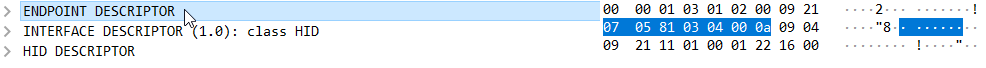
\includegraphics[width=\textwidth]{img/uvod_wireshark_tree_click}
	\caption{Ukážka kliknutia na položku \textit{endpoint descriptoru} v stromovej štruktúre.}
	\label{obr:uvod:tree_click}
\end{figure}

Obecné vyobrazenie pohybu paketov na zbernici bez hlbšej analýzy je ukázané na obrázku~\ref{obr:uvod:wireshark_listview} nižšie.

\begin{figure}[!htb]
	\centering
	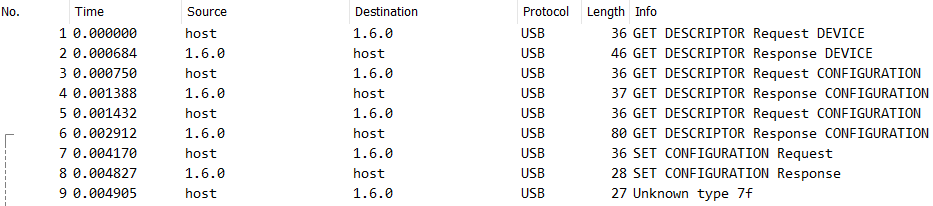
\includegraphics[width=\textwidth]{img/uvod_wireshark_listview}
	\caption{Príklad obecného vyobrazenia jednotlivých paketov vo Wiresharku.}
	\label{obr:uvod:wireshark_listview}
\end{figure}

Výhoda Wiresharku je hlavne v~tom, že podporuje širokú škálu descriptorov a~plná verzia programu je dostupná úplne zadarmo. Z~pohľadu užívateľa je až prekvapivé, že aj~napriek rozsiahlosti programu je aplikácia veľmi user-friendly orientovaná a~dopĺňa ju intuitívne užívateľské rozhranie.

Naopak, jeho nevýhodou je sčasti neprehľadný hexdump. Ako môžeme vidieť na obrázku~\ref{obr:uvod:wireshark_hexdump}, jedná sa o obyčajný hexdump, ktorý nijakým spôsobom neoddeľuje význam dát bez interakcie užívateľa. Preto v momente ak by sme nemali stromovú štruktúru k odpovedajúcemu hexdumpu, museli by sme sa riadiť špecifikáciou a vlastnou analýzou. V prípade rozsiahlejšieho hexdumpu môže byť veľmi obtiažné sa v ňom potom zorientovať. Ďalšia vec ktorá nám nevyhovuje, je chýbajúca sémantická analýza inputu rôznych zariadení. Ten je vyobrazený len pomocou hexdumpu a popisu \uv{Leftover Capture Data} ako je ukázané na obrázku~\ref{obr:uvod:wireshark_input}~\footnote{V čase dokončovania tejto práce bola k dispozícii verzia Wiresharku 3.4.5, ktorá ponúkala sémantickú analýzu inputu HID zariadení.}. Zo sekcie~\ref{uvod:sec:HID} nám je teda jasné, že vôbec netušíme čo jednotlivé dáta znamenajú, pretože ich význam je definovaný v \textit{Report Descriptore}.

\begin{figure}[!htb]
	\centering
	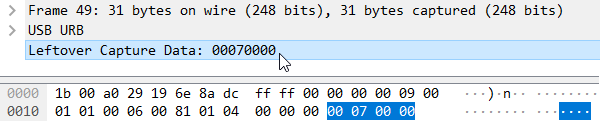
\includegraphics[width=12cm]{img/uvod_wireshark_input}
	\caption{Príklad inputu myši vo Wiresharku.}
	\label{obr:uvod:wireshark_input}
\end{figure}

\subsection*{Device Monitoring Studio}

Aplikácia ponúka analýzu sieťových a~USB paketov, tak ako aj~analýzu komunikácie prebiehajúcej cez~sériový port. Zároveň slúži aj ako sniffer na všetkých týchto portoch.

Ako prvé na~aplikácii zaujme spôsob zvolenia si zariadenia s~ktorým bude sledovaná komunikácia. Je implementovaný štýlom stromovej štruktúry ako je ukázané na~obrázku~\ref{obr:uvod:hhd_treeview_foto}~nižšie, kde máme konkrétne označenú rovnakú myš s ktorou komunikáciu sme sledovali predchádzajúcim programom~\footnote{Verzia programu použítá v tejto sekcii na priblíženie jeho funkcionality je 8.36.00.9618}. 

\begin{figure}[!htb]
	\centering
	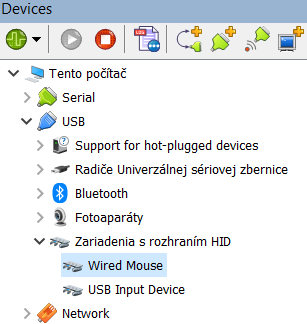
\includegraphics{img/uvod_hhd_treeview}
	\caption{Ukážka stromovej štruktúry na~zvolenie si zariadenia, s~ktorým bude zachytávaná komunikácia.}
	\label{obr:uvod:hhd_treeview_foto}
\end{figure}
\newpage
Základná verzia programu ponúka vizuálne zobrazenie \textit{URB}, tak ako aj analýzu jednotlivých paketov.
Pod analýzou si tu môžeme predstaviť ale len obyčajný hexdump, ktorý neposkytuje žiadne významové oddelenie dát a tým pádom je obtiažnejšie sa v ňom zorientovať. Príklad môžeme vidieť na obrázku~\ref{obr:uvod:hhd_hexdump}.

\begin{figure}[!htb]
	\centering
	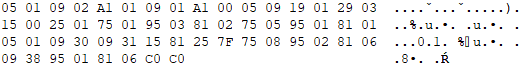
\includegraphics[width=12cm]{img/uvod_hhd_hexdump}
	\caption{Príklad hexdumpu v Device Monitoring Studio.}
	\label{obr:uvod:hhd_hexdump}
\end{figure}


Takisto tu nemáme kompletné sémantické vysvetlenie čo dané dáta znamenajú (napríklad pomocou stromovej štruktúry ako to rieši konkurencia). K dispozícii máme len veľmi obmedzený popis jednotlivých paketov (číslo paketu, device request, a pod.), pričom ani nie je veľmi jasné odkiaľ sa tieto informácie vzali. Príklad takéhoto popisu aj s hexdumpom je ukázaný na obrázku~\ref{obr:uvod:hhd_analyza}~nižšie.

\begin{figure}[!htb]
	\centering
	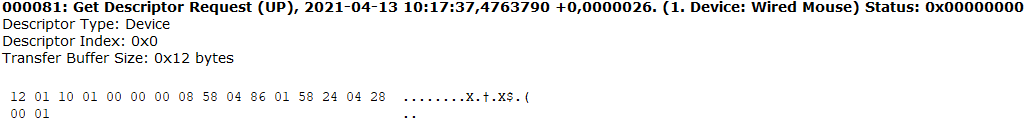
\includegraphics[width=\textwidth]{img/uvod_hhd_analyza}
	\caption{Príklad analýzy paketov.}
	\label{obr:uvod:hhd_analyza}
\end{figure}


Vyobrazenie \textit{URB} (obrázok~\ref{obr:uvod:hhd_urb}~) tak ponúka súhrn týchto popisov jednotlivých paketov, ktoré sú postupne zachytené počas komunikácie na zbernici.

\begin{figure}[!htb]
	\centering
	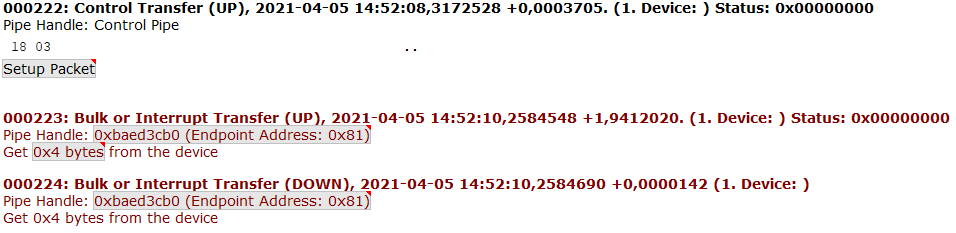
\includegraphics[width=\textwidth]{img/uvod_hhd_urb}
	\caption{Ukážka vyobrazenia URB.}
	\label{obr:uvod:hhd_urb}
\end{figure}

Pričom pri dvojkliku na šedé časti textu (napríklad \textit{Setup Packet} alebo \textit{Endpoint Address}) sa užívateľovi rozbalí okno s detailnejším popisom.
 
Analýza inputu myši, ktorú môžeme vidieť na obrázku~\ref{obr:uvod:hhd_input}, je riešená podobným spôsobom ako pri analýze descriptorov.

\begin{figure}[!htb]
	\centering
	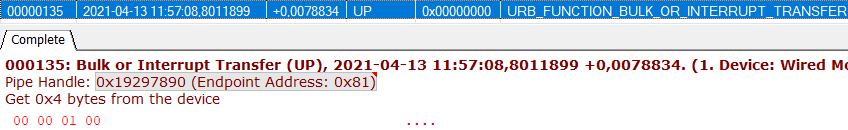
\includegraphics[width=\textwidth]{img/uvod_hhd_input}
	\caption{Príklad inputu myši v Device Monitoring Studio.}
	\label{obr:uvod:hhd_input}
\end{figure}

Obecné vyobrazenie jednotlivých paketov bez bližšej analýzy je riešené podobne ako vo Wiresharku, pričom pakety sú farebne oddelené podľa ich smeru pohybu na zbernici (posielané smerom host $\longrightarrow$ zariadenie/smerom zariadenie $\longrightarrow$ host). Toto je veľmi pekná funkcionalita, ktorá celkovo sprehľadňuje komunikáciu zariadenia s hostom. Príklad je ukázaný na obrázku~\ref{obr:uvod:hhd_listview}.

\begin{figure}[!htb]
	\centering
	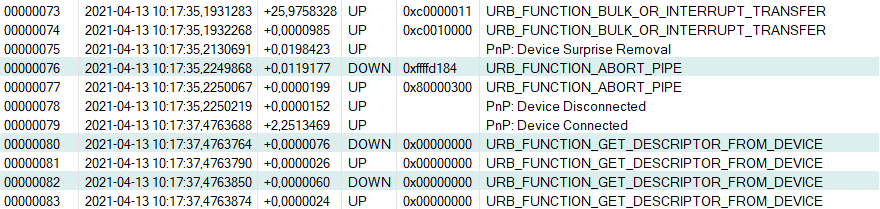
\includegraphics[width=\textwidth]{img/uvod_hhd_listview}
	\caption{Príklad obecného vyobrazenia jednotlivých paketov v Device Monitoring Studio.}
	\label{obr:uvod:hhd_listview}
\end{figure}

Zaujímavá funkcionalita, ktorú ale program ponúka len v platenej verzii, je umožnenie užívateľovi priamo komunikovať so zvoleným zariadením. Môžeme mu tak posielať rôzne požiadavky (niektoré z nich sú spomenuté v USB 2.0 špecfikácii\cite{usbdoc} v kapitole 9.4) ako napríklad \textit{GET\_REPORT} kde špecifikujeme \textit{Report ID} a prípadné ďalšie parametre, a zariadenie nám patrične odpovie.

Užívateľské rozhranie vyobrazené nižšie pomocou obrázku~\ref{obr:uvod:hhd_interface}~,pozostáva z pomerne veľa ikoniek a celkovo sa javí ako trochu neprehľadné. Pri prvotnej interakcii s programom chvíľu trvá, kým človek nájde čo~i~len základné informácie ako napríklad hlavičky ku~jednotlivým paketom. Nepoteší ani fakt, že verzia zadarmo nedovoľuje monitorovanie dlhšie ako 10 minút a~maximálny počet monitorovaní za~jeden deň je taktiež 10.

\begin{figure}[!htb]
	\centering
	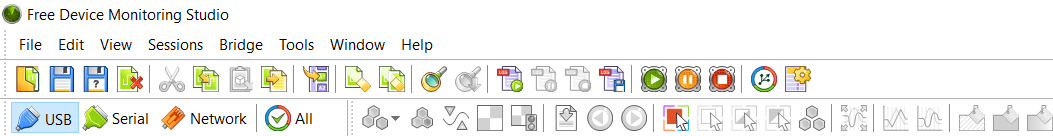
\includegraphics[width=\textwidth]{img/uvod_hhd_interface}
	\caption{Užívateľské rozhranie Device Monitoring Studio.}
	\label{obr:uvod:hhd_interface}
\end{figure}


\section{Požadované funkcie}

Ako prvé by sme si mali zadefinovať platformu na ktorú budeme cieliť s našou aplikáciou:
\begin{enumerate}[label=\textbf{P\arabic*}]
	\item \label{uvod:poz:platforma} Cieľová platforma našej aplikácie by mala byť Windows. 
\end{enumerate}

Keďže má naša aplikácia mať výukový charakter, tak sa pozrieme na typický výukový scénár jej používania. Učiteľ si dopredu do súboru zachytí komunikáciu s určitým zariadením na ktorej overí, že je didakticky dobrá a ilustruje to čo má. Následne daný súbor posunie študentom aby si mohli zobraziť analýzu konkrétnych paketov. Užitočná je ale aj analýza priamej interakcie užívateľa s jeho konkrétnym zariadením, preto by sme zároveň chceli podporovať aby si študenti mohli pripojiť vlastné zariadenie a skúmať s ním komunikáciu v reálnom čase. Z toho nám vyplývajú naledujúce požiadavky:
\begin{enumerate}[label=\textbf{P\arabic*},resume]
	\item \label{uvod:poz:analyza} Mala by byť schopná analyzovať USB pakety zachytené do~súboru v~rozumnom formáte pomocou predom definovaného snifferu.
	\item \label{uvod:poz:analyza_real_time} Mala by byť schopná analýzy paketov v reálnom čase. To znamená, že bude podporovať čítanie súboru súvisle s tým ako do neho bude zapisovať iný software (za predpokladu, že to daný software povoľuje).
\end{enumerate}

Ako sme mohli vidieť aj na predchádzajúcich príkladoch, hexdump je jednou zo základných funkcií na analýzu paketov. Zároveň sa nám ale nepáčilo, že väčšina hexdumpov je neprehľadná a ťažko sa v nich orientuje. Preto si zadefinujeme nasledujúce požiadavky:
\begin{enumerate}[label=\textbf{P\arabic*},resume]
	\item \label{uvod:poz:hexdump} Mala by pomocou hexdumpu vedieť zobraziť dáta, ktoré daný sniffer zachytí a~uloží.
	\item \label{uvod:poz:data_highlight} Mala by mať prehľadnejší hexdump a užívateľovi uľahčiť orientáciu v~ňom. Jednotlivé znaky by mali byť farebne označené na~základe ich významu (hlavička paketu, rôzne typy descriptorov a pod.).
\end{enumerate}

K sémantickej analýze sa nám môže hodiť vedieť zobraziť dáta a ich význam pomocou stromovej štruktúry. Pretože sa s našou aplikáciou budeme snažiť vysvetliť základy komunikácie na USB zbernici, mali by sme podporovať sémantickú analýzu všetkých základných USB descriptorov a takisto inputu určitej podmnožiny HID zariadení. Ako posledné by sa nám zišlo vedieť pomocou stromovej štruktúry vyobraziť hlavičku jednotlivých paketov. Z toho celého dostávame nasledovné:
\begin{enumerate}[label=\textbf{P\arabic*},resume]
	\item \label{uvod:poz:descriptory} Mala by podporovať sémantickú analýzu (vyobrazenie pomocou stromovej štruktúry) pre~všetky základné USB descriptory spomenuté v~USB 2.0 špecifikácii~\cite{usbdoc} v kapitole 9.6~(ako napríklad \textit{Device descriptor}, \textit{Interface descriptor}, \textit{Endpoint descriptor}, atď.).
	\item \label{uvod:poz:hid_analyza} Mala by byť schopná pomocou stromovej štruktúry zobraziť sémantický význam dát posielaných danou podmnožinou HID zariadení, do~ktorej patrí myš, klávesnica a~joystick.
	\item \label{uvod:poz:paket_hlavicka} Mala by byť schopná pomocou stromovej štruktúry zobraziť sémantický význam jednotlivých hlavičiek paketov.
\end{enumerate}

Vyššie v texte sme označili funkciu Wiresharku vyobraziť sémantický význam dát na bitovej úrovni (obrázok~\ref{obr:uvod:byte_detail_foto}) za zaujímavú. Preto by sme ju chceli implementovať aj v našej aplikácii, z čoho vyplýva:
\begin{enumerate}[label=\textbf{P\arabic*},resume]
\item \label{uvod:poz:show_bits} V~miestach kde to dáva zmysel, by aplikácia mala byť schopná zobrazovať význam dát až na~úrovni jednotlivých bitov.
\end{enumerate}

Nechceme užívateľov hneď zaplaviť všetkými detailnými informáciami o paketoch. Preto by sme mali vedieť zobraziť zopár obecných vecí ku každému paketu a vyobraziť tak pohyb na zbernici, a až v prípade interakcie užívateľa s aplikáciou zobraziť podrobný popis jednotlivých paketov. Zároveň sa nám páčila funkcia Device Monitoring Studia, kde boli jednotlivé pakety farebne rozlišiteľné, čo zvyšovalo celkový prehľad pohybu paketov na zbernici. Z toho dostávame nasledujúce požiadavky:
\begin{enumerate}[label=\textbf{P\arabic*},resume]
	\item \label{uvod:poz:zobrazenie_paketov} Mala by na prvý pohľad jasne zobraziť základné informácie o~každom analyzovanom pakete (ako napr. dĺžka paketu, typ prenosu a pod.) a~pri~bližšom skúmaní jednotlivých paketov detailnejšie zobraziť celú jeho hlavičku. Tieto základné informácie by mali byť farebne rozlišiteľné na základe smeru paketu po zbernici.
	\item \label{uvod:poz:paket_detail} Detailnejšie informácie o~pakete budú zobrazované na~základe interakcie užívateľa s~aplikáciou.
\end{enumerate}

Aby sme boli schopní sémantickej analýzy dát myši, klávesnice alebo joysticku podľa osobného výberu užívateľa, musíme si získať informácie o ich inpute z \textit{HID Report Descriptoru}, takže naša ďalšia požiadavka je:
\begin{enumerate}[label=\textbf{P\arabic*},resume]
	\item \label{uvod:poz:report_desk_parser} Mala by byť schopná rozparsovať \textit{HID Report Descriptor} takým štýlom, aby bolo neskôr možné sématnicky reprezentovať input nami zvolených HID zariadení -- myš, klávesnica a joystick.
\end{enumerate}

\section{Ciele práce}

Celkové ciele tejto práce sú následovné :

\begin{enumerate}[label=\textbf{C\arabic*}]
	\item \label{uvod:ciel:aplikacia} Naprogramovať funkčný analyzátor, ktorý spĺňa všetky požadované funkcie~\ref{uvod:poz:platforma}\=/\ref{uvod:poz:report_desk_parser}
	\item \label{uvod:ciel:rozsiritelnost} Návrh programu musí byť dostatočne obecný aby splňoval nasledujúce:
	\begin{itemize}
		\item \label{uvod:ciel:roz_USB} Jednoduché rozšírenie o~analýzu ďalších typov USB prenosov.
		\item \label{uvod:ciel:roz_HID} Jednoduché pridanie sémantickej analýzy pre~ďalšie HID zariadenia.
	\end{itemize}
\end{enumerate}